%*****************************************************************
%*************************** Section 3 ***************************
%************* Controllerplatine und Programmiertool *************
%*****************************************************************


\pagestyle{fancy}
\rhead{\thepage} \chead{} \lhead{\ref{Sec3}. \nameref{Sec3}}
\cfoot{}

\section{Controllerplatine und Programmiertool}\label{Sec3}

Für dieses Projekt wird die Controllerplatine LPCXpresso54628 von NXP Semiconductors verwendet. Das Herzstück dieser Platine ist der auf dem ARM Cortex-M4 basierende Mikrocontroller LPC54628. Dieser Controller wird wegen seiner schnellen Taktfrequenz und seiner großen Anzahl an Peripherie für die Ansteuerung der Motoren und des Servos sowie für die Sensorik zur Bestimmung des Streckenverlaufs verwendet. Der Vorteil einer fertigen Controllerplatine liegt darin, dass der Schaltplan sowie das dazugehörige Layout professionell erstellt sind, wodurch dieser aufwendige Schritt bei der Entwicklung des Autos entfällt und die einwandfreie Funktionsweise des Controllers sichergestellt wird. Außerdem ist darauf bereits ein Debugger zur Programmierung und Fehlersuche verbaut. Durch das Flashen dieses Debuggers über das Programm \glqq{}LPCScrypt\_2.1.2\_57\grqq{} kann zwischen dem J-Link Debugger (Standardinstallationspfad + scripts/program\_JLINK.cmd) und dem NXP-eigenen LinkServer Debugger (Standardinstallationspfad + scripts/program\_CMSIS.cmd) gewählt werden. 

\begin{figure}[H] %H für Positionierung hier
	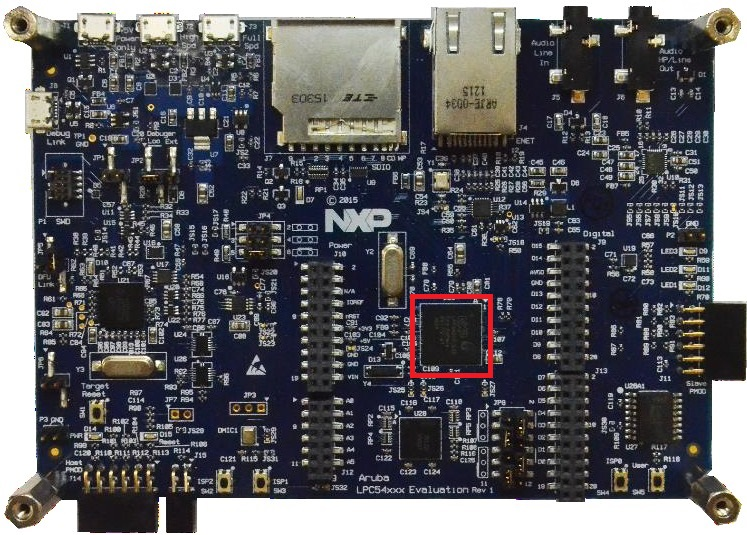
\includegraphics[width=.80\textwidth]{sec3/images/Controllerplatine} 
	\centering
	\captionsetup{width=.95\textwidth}
	\caption[Controllerplatine LPCXpresso54628 ~\protect\cite{Semic}]{Draufsicht auf die Controllerplatine mit dem Mikrocontroller LPC54628  (in rot hervorgehoben) als Hauptbestandteil ~\protect\cite{Semic}}\centering
	\label{fig:Controllerplatine}
\end{figure}

Zur Programmierung des Controllers dient das auf Eclipse basierende Tool \glqq{}MCUXpresso\grqq{}, welches von NXP Semiconductors zur Verfügung gestellt wird. Darin sind die für den verwendeten Controller notwendigen Konfigurationsdateien, wie beispielsweise das Startup-Skript und einige Beispiele, bereits enthalten. Das erleichtert den Einstieg in die Programmierung erheblich. Außerdem kann das Konfigurationstool \glqq{}MCUXpresso Config Tools\grqq{} verwendet werden. Mit diesem kann die Initialisierung der Peripheriebausteine über eine graphische Benutzeroberfläche vorgenommen werden.

\newpage